
%%%%%%%%%%%%%%%%%%%%%%%%%%%%%%%%%%%%%%%%%%%%%%%%%%%%%%%%%%%%%%%%%%%%%%%%
%Para las ecuaciones siempre es Ec.(n).
%Para las figuras siempre es Fig.n, incluso en el caption de la figura. Tambien las Tablas
%Para las referencias es [n]
%%%%%%%%%%%%%%%%%%%%%%%%%%%%%%%%%%%%%%%%%%%%%%%%%%%%%%%%%%%%%%%%%%%%%%%%

\documentclass[
reprint,
%notitlepage,
%superscriptaddress,
%groupedaddress,
%unsortedaddress,
%runinaddress,
%frontmatterverbose, 
%preprint,
%showpacs,preprintnumbers,
%nofootinbib,
%nobibnotes,
%bibnotes,
%11 pt,
amsmath,
amssymb,
aps,
%pra,
%prb,
%rmp,
%tightenlines %esto hizo el milagro de sacar los espacios en blancos estocásticos (?)
 %prstab,
%prstper,
%floatfix,\textbf{}
]{revtex4-1} %Instalar primero para usarlo. Paquete malo.

%\documentclass[onecolumn, aps, amsmath,amssymb ]{article}
\usepackage{lipsum}  
\usepackage{graphicx}% Include figure files
\usepackage{subfig}
\usepackage{braket}
\usepackage{comment} %comment large chunks of text
\usepackage{dcolumn}% Align table columns on decimal point
\usepackage{bm}% bold math
%\usepackage{hyperref}% add hypertext capabilities
\usepackage[mathlines]{lineno}% Enable numbering of text and display math
%\linenumbers\relax % Commence numbering lines
\usepackage{mathtools} %% Para el supraíndice

\usepackage[nice]{nicefrac}

%%%%%%%El Señor Español%%%%%%%%%%%%%%%%%%%%%%%%%%%
\usepackage[utf8]{inputenc} %acento
\usepackage[
spanish, %El lenguaje.
es-tabla, %La tabla y no cuadro.
activeacute, %El acento.
es-nodecimaldot %Punto y no coma con separador de números
]{babel}
\usepackage{microtype} %para hacerlo más bonito :33 como vos (?) 
%%%%%%%%%%%%%%%%%%%%%%%%%%%%%%%%%%%%%%%%%%%%%%%%%%%
%%%%%%%%% Para que las imágenes se queden dónde las quiero (?
\usepackage{float}
%%%%%%%%%%

%%%%%%%%Cambia a Fig de Figure%%%%%%%%%%
\makeatletter
\renewcommand{\fnum@figure}{Fig. \thefigure} 
\makeatother
%%%%%%%%%%%%%%%%%%%%%%%%%%%%%%%%%%%%%%%%
\raggedbottom


\begin{document}
%%%%%%%%%%%%%%%%%%%%%%%%%%%%%%%%%%Título%%%%%%%%%%%%%%%%%%%%%%%%%%%%%%%%%%%%%%
%%%%%%%%%%%%%%%%%%%%%%%%%%%%%%%%%%%%%%%%%%%%%%%%%%%%%%%%%%%%%%%%%%%%%%%%%%%%%%

\title{Reconstrucción de energía}
\author{Evelyn~G.~Coronel}

\affiliation{
Tesis de Maestría en Ciencias Físicas\\ Instituto Balseiro\\}

\date[]{\lowercase{\today}} %%lw para lw, [] sin date

%\begin{abstract}

%\end{abstract} 
\maketitle


\subsection{Rango de tiempo}
\begin{table}[H]
\centering
\begin{tabular}{c|c|c}
Inicio & 1388628499 & 2 January 2014 \\ \hline
Final  & 1550534100 & 18 February 2019 \\
\end{tabular}
\end{table}

\subsection{Tasa de eventos}

\begin{figure}[H]
	\centering
	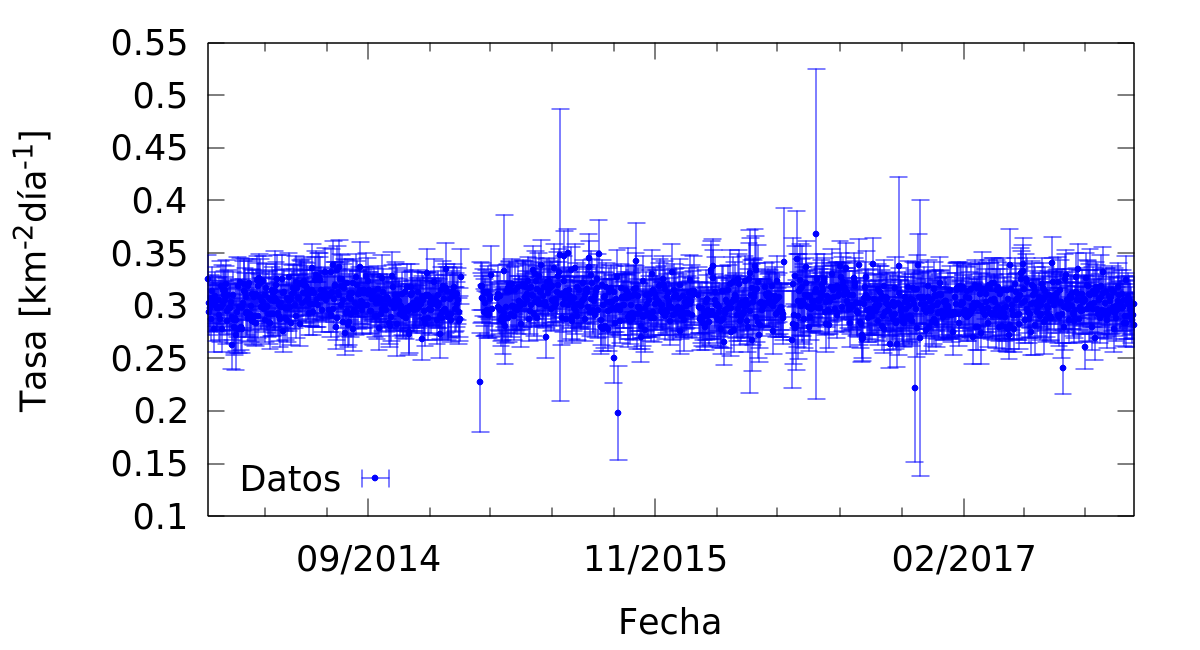
\includegraphics[width=0.5\textwidth]{rate_1_EeV.png}
\end{figure}

Antes del 2 de Enero del 2014, se tenía una tasa por debajo de la media de los siguientes años.


\subsection{Párametros del clima}

\begin{figure}[H]
	\centering
	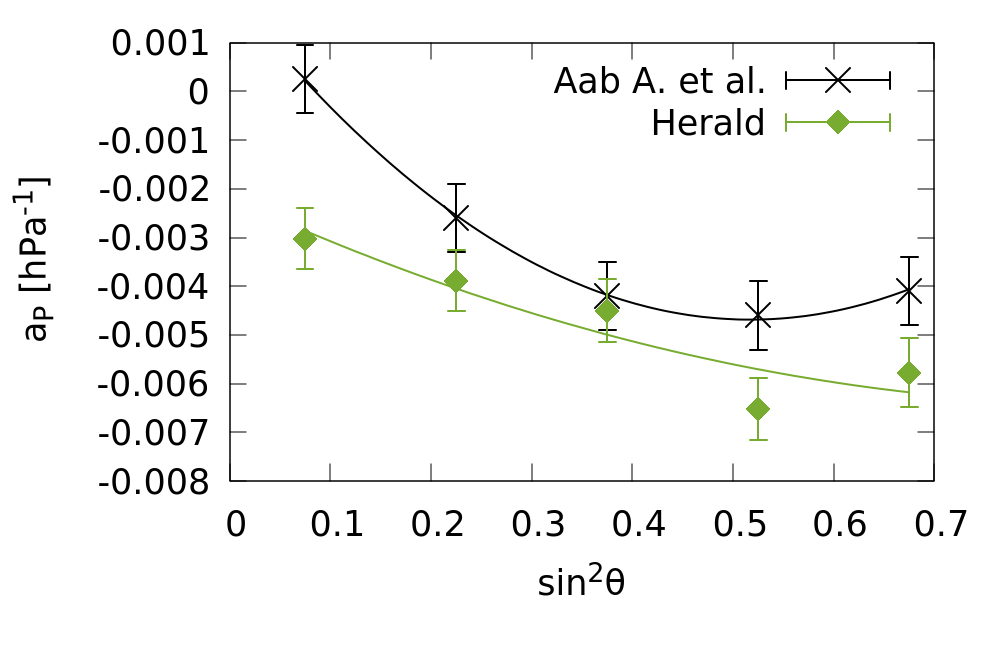
\includegraphics[width=0.5\textwidth]{ap.png}
\end{figure}


\begin{figure}[H]
	\centering
	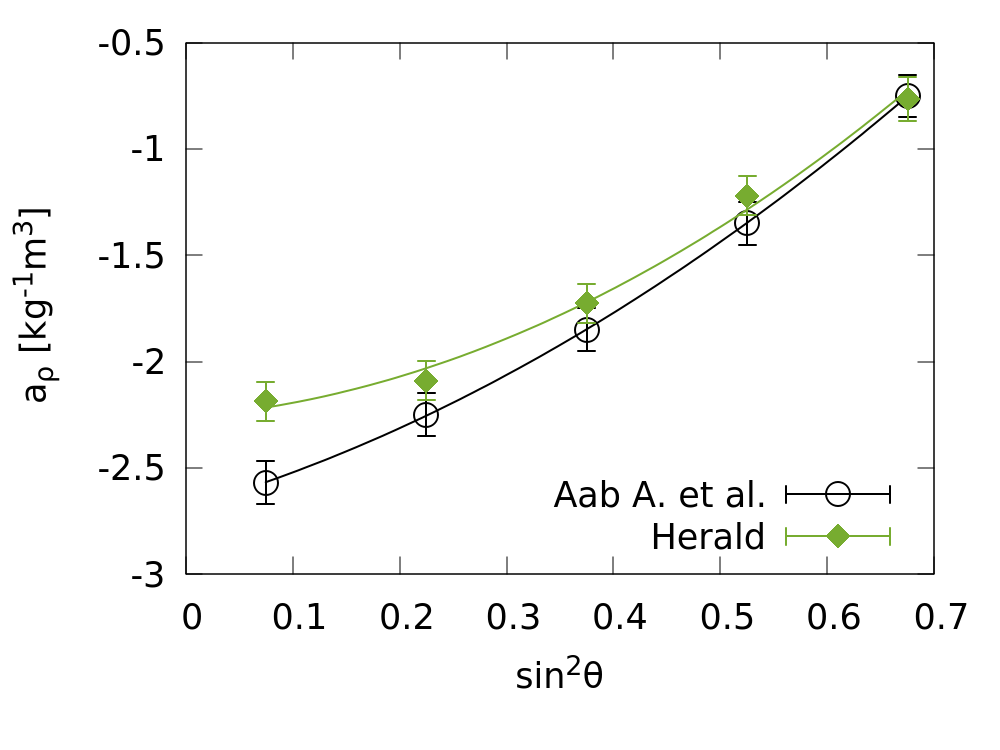
\includegraphics[width=0.5\textwidth]{arho.png}
\end{figure}


\begin{figure}[H]
	\centering
	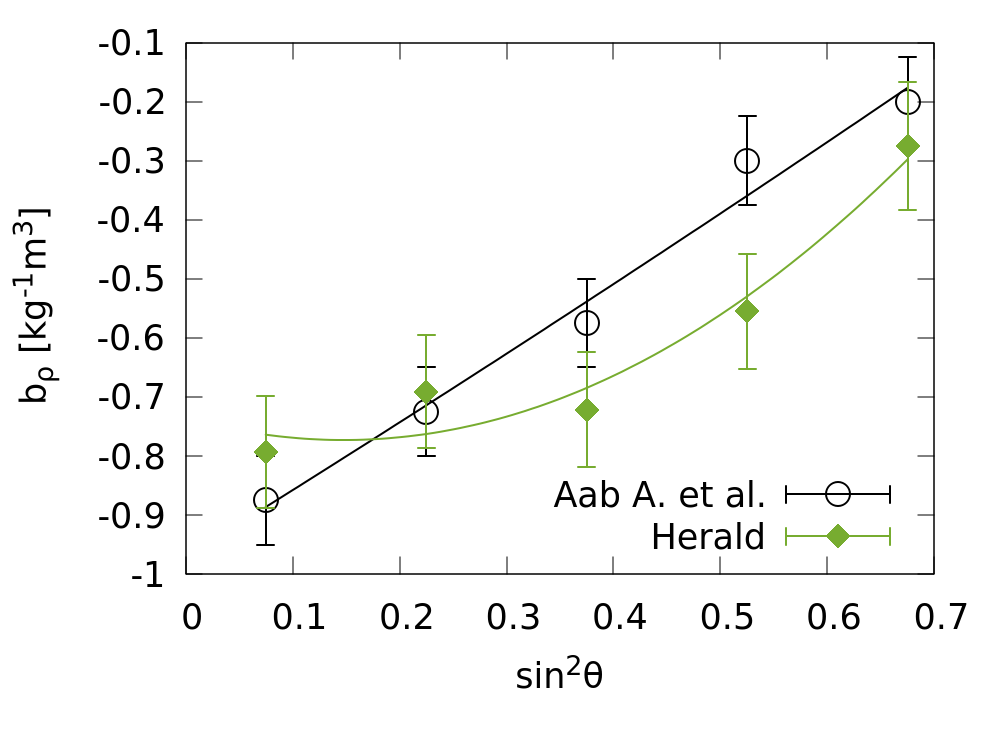
\includegraphics[width=0.5\textwidth]{brho.png}
\end{figure}

Considerando una cuádrica para el ajuste de la curva, se obtiene los parámetros de la siguiente table
\begin{table}[H]
\centering
\begin{tabular}{c|c|c|c}
		 	& $a_P$ 	&  $a_\rho$  & $ b_\rho$ \\ \hline
$c_0$ 		& -0.002(1) & 	-2.2(1)	 &	-0.74(9)\\ \hline
$c_1$ 		& -0.009(6)	& 	 0.4(6)	 &	-0.0(6)\\ \hline
$c_2$ 		&  0.00(9) 	& 	 2.7(8)  &	 1.7(7)\\ \hline
\end{tabular}
\end{table}


\subsection{Anisotropía en el rango 1-2 EeV}

\begin{figure}[htbp]
	\centering
	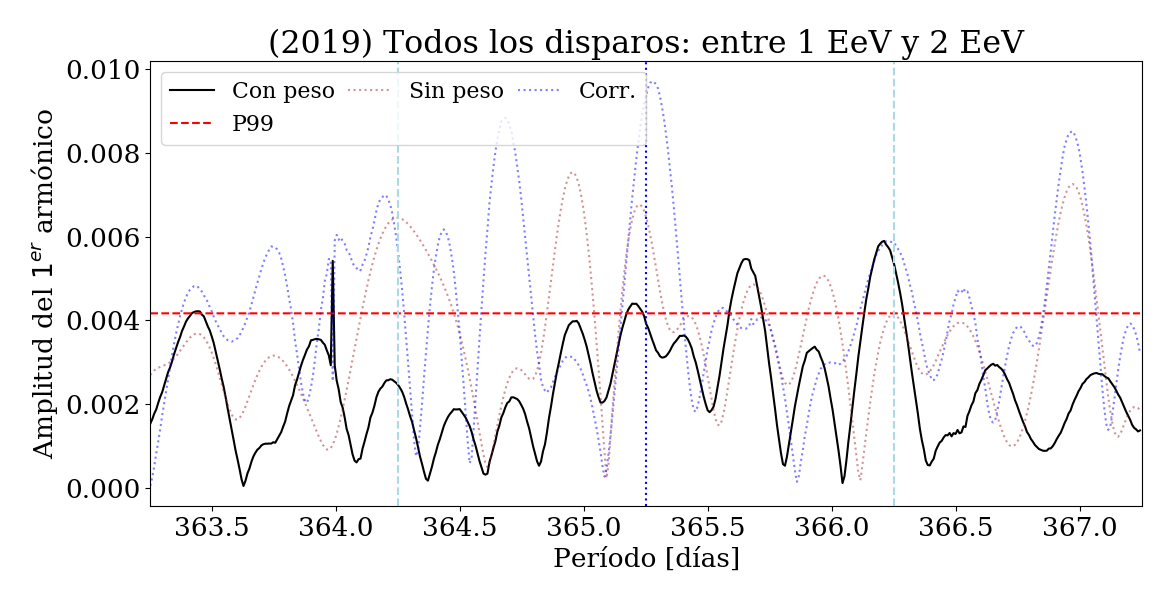
\includegraphics[width=0.5\textwidth]{ani_corr.png}
\end{figure}



\end{document}